% Slide 19: Detecção de Comunidades
\begin{frame}{Detecção de Comunidades}
    \begin{block}{Comunidades Revelam Eras Históricas}
        \footnotesize
        \begin{itemize}
            \item Algoritmo Louvain identifica agrupamentos naturais
            \item \textbf{Eras da Guerra Fria:} USA vs USSR (Basquete M)
            \item \textbf{Pós-colapso USSR:} redistribuição de atletas (1992+)
            \item \textbf{Hegemonias regionais:} Brasil (Futebol), Japão (Judô), Jamaica (Atletismo)
        \end{itemize}
    \end{block}

    \vspace{0.3cm}

    \begin{block}{Hierarquia de Perfis}
        \footnotesize
        \begin{description}
            \item[\textbf{Núcleo:}] Atletas com múltiplas medalhas, alta centralidade, conectados entre si
            \item[\textbf{Intermediária:}] Atletas com 2-3 medalhas, ponte entre núcleo e periferia
            \item[\textbf{Periferia:}] Atletas com 1-2 medalhas, baixa conectividade
        \end{description}
    \end{block}

    \vspace{0.3cm}

    \begin{block}{Métricas de Diversidade}
        \footnotesize
        \begin{itemize}
            \item \textbf{Entropia Temporal:} mede distribuição de atletas ao longo do tempo
            \item \textbf{Entropia Geográfica:} mede diversidade de países em comunidade
        \end{itemize}
    \end{block}
\end{frame}

% Slide 20: Evolução Temporal
\begin{frame}{Evolução Temporal das Redes}
    \begin{columns}[T]
        \begin{column}{0.50\textwidth}
            \begin{center}
                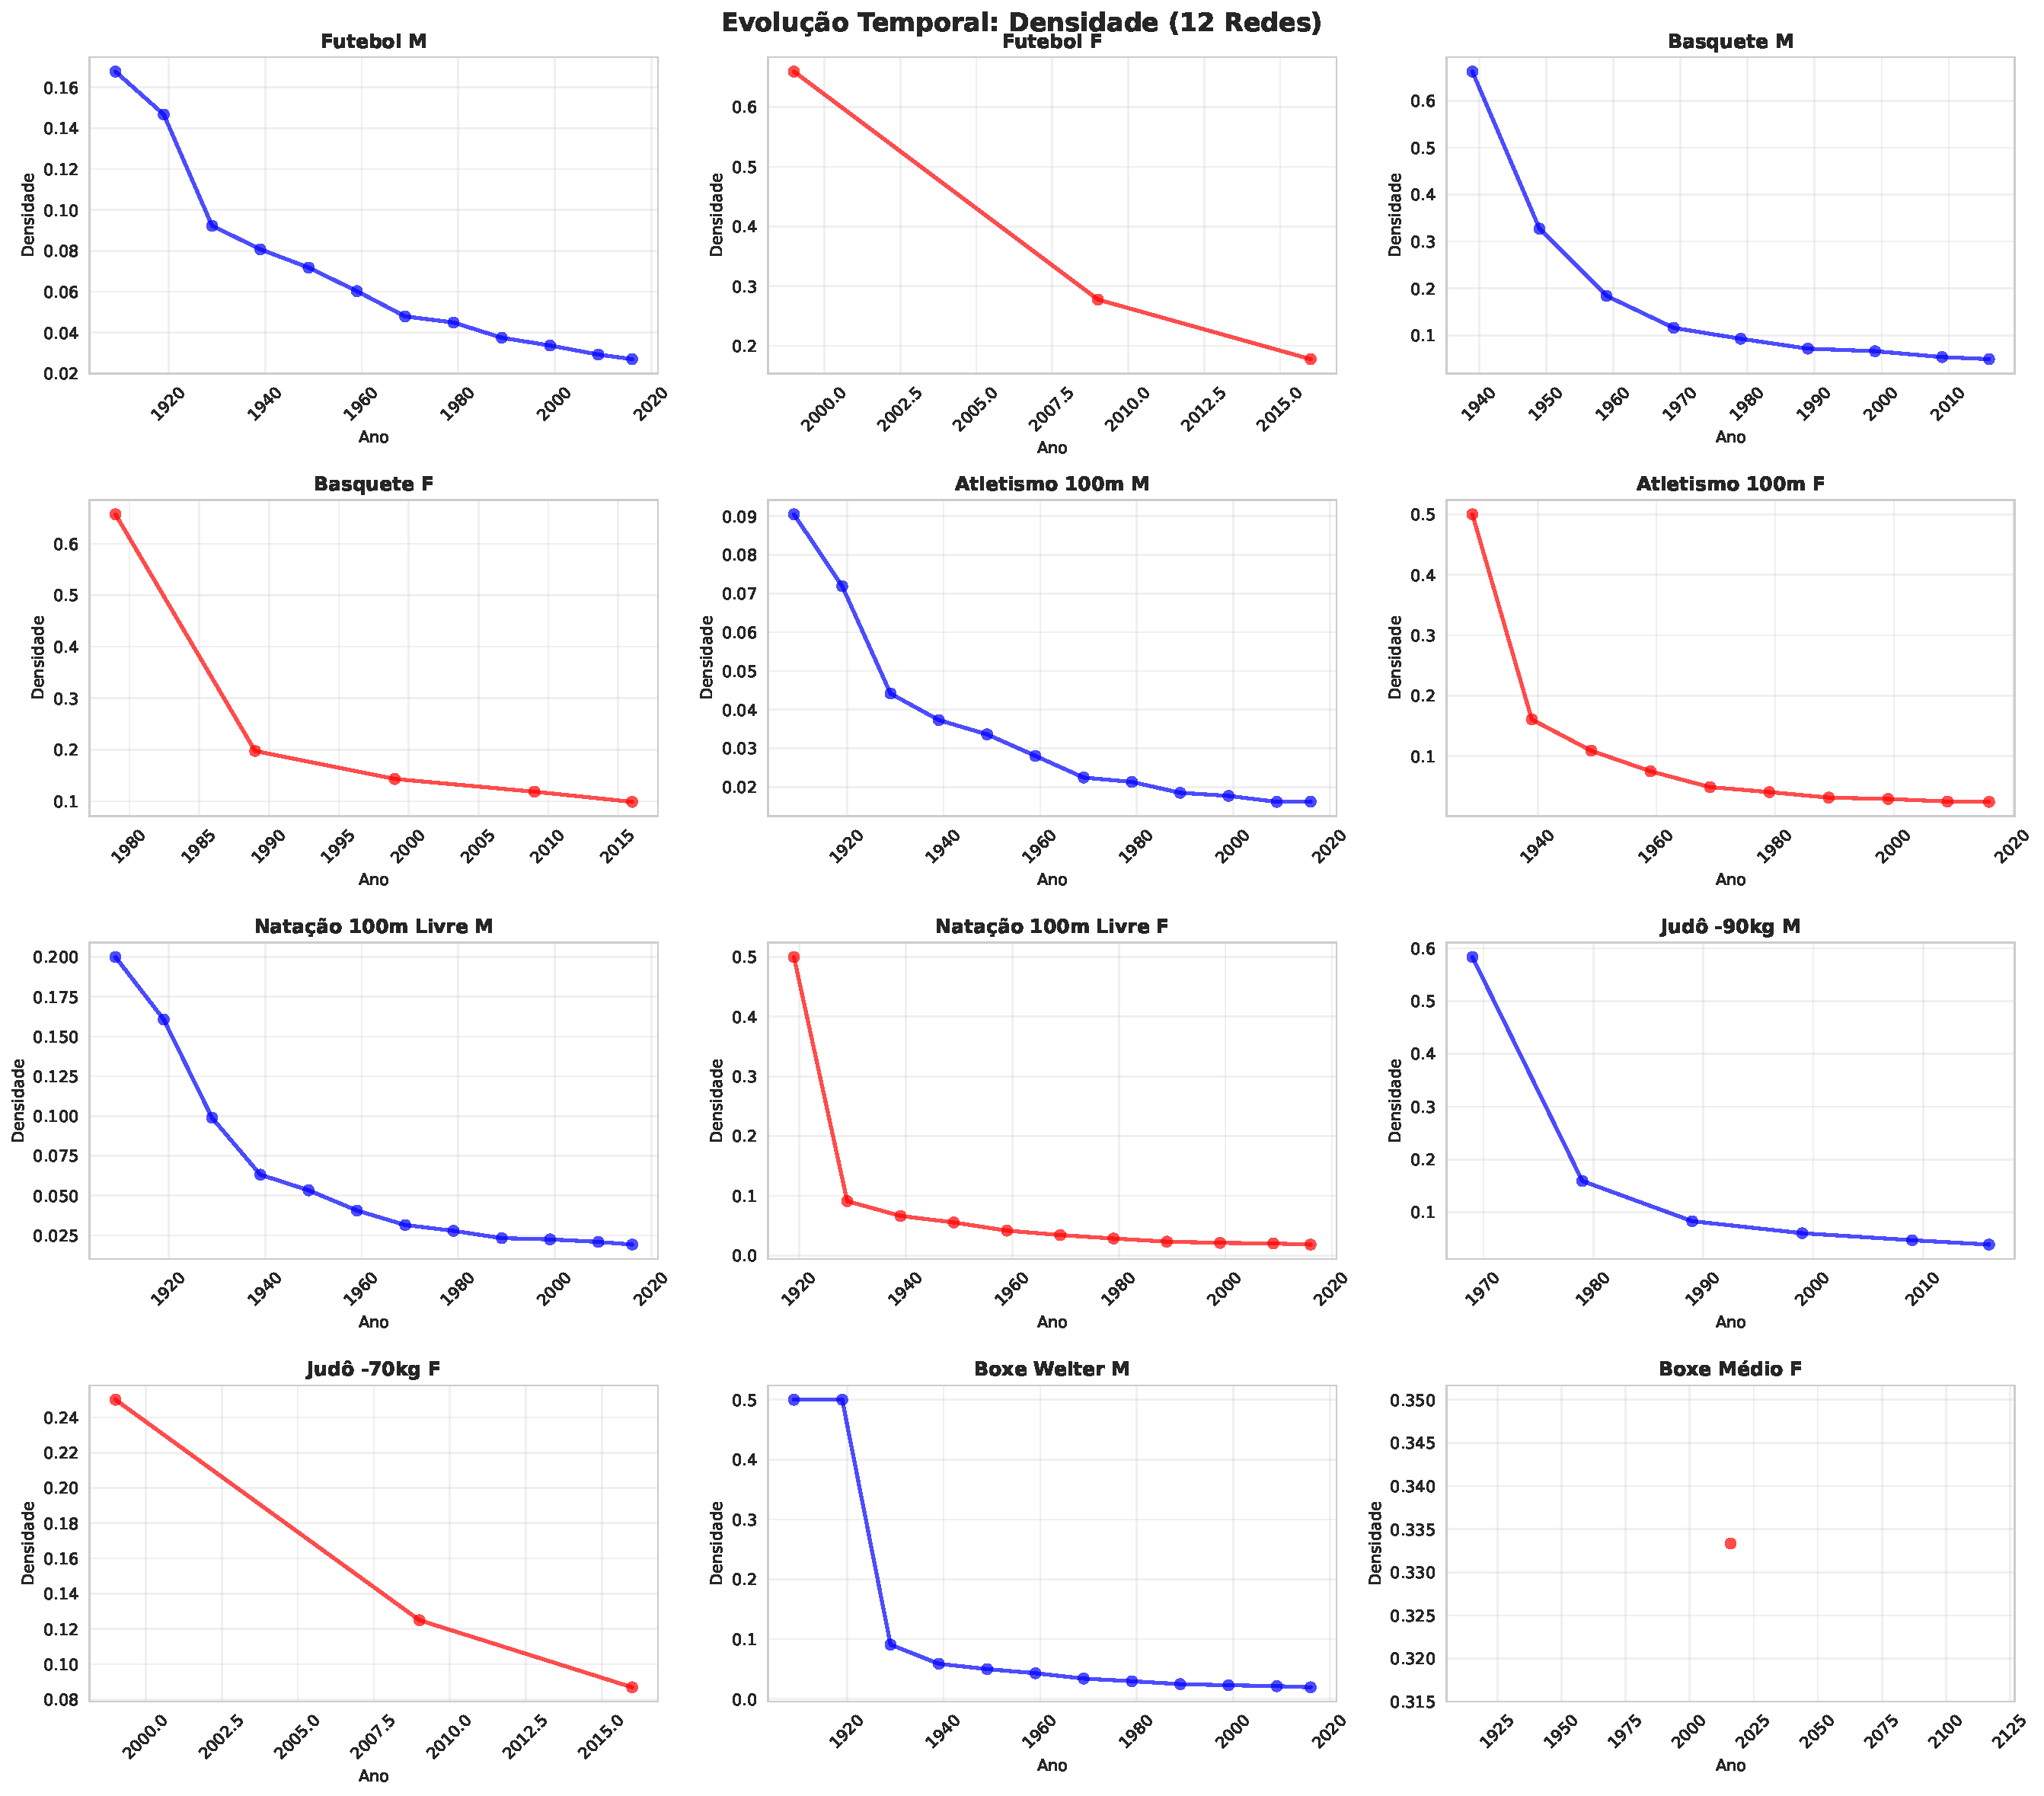
\includegraphics[width=\textwidth]{../monografia/figuras/temporal_evolution_density.pdf}\\
                \vspace{0.1cm}
                \footnotesize\textit{Densidade decresce com o tempo}
            \end{center}
        \end{column}
        \begin{column}{0.48\textwidth}
            \begin{block}{Densidade Decrescente}
                \footnotesize
                \begin{itemize}
                    \item Primeiras Olimpíadas: alta densidade\\(poucos competidores)
                    \item Olimpíadas modernas: mais atletas, mais especialização
                \end{itemize}
            \end{block}
            \vspace{0.2cm}
            \begin{block}{Modularidade Resiliente}
                \footnotesize
                \begin{itemize}
                    \item \textbf{Q $>$ 0.60} mantido ao longo de 120 anos
                    \item Estrutura competitiva estável apesar de mudanças geopolíticas
                \end{itemize}
            \end{block}
            \vspace{0.2cm}
            \begin{alertblock}{}
                \footnotesize\centering
                Padrões estruturais são \textbf{robustos}
            \end{alertblock}
        \end{column}
    \end{columns}
\end{frame}

% Slide 21: Descoberta Contra-Intuitiva: Especialização em Ouro
\begin{frame}{Descoberta: Especialização em Ouro na Periferia}
    \begin{block}{Padrão Contra-Intuitivo}
        \Large
        \centering
        Atletas periféricos têm \textbf{maior \% de ouros}
    \end{block}

    \vspace{0.5cm}

    \begin{columns}[T]
        \begin{column}{0.48\textwidth}
            \begin{block}{Núcleo}
                \footnotesize
                \begin{itemize}
                    \item Múltiplas medalhas
                    \item Balanceamento: ouros, pratas, bronzes
                    \item Exemplos: Phelps, Bolt
                    \item Carreira longa
                \end{itemize}
            \end{block}
        \end{column}
        \begin{column}{0.48\textwidth}
            \begin{block}{Periferia}
                \footnotesize
                \begin{itemize}
                    \item 1-2 medalhas apenas
                    \item \textbf{Alta \% de ouros}
                    \item Especialização extrema
                    \item "One-hit wonders"
                \end{itemize}
            \end{block}
        \end{column}
    \end{columns}

    \vspace{0.3cm}

    \begin{center}
        \footnotesize
        \textit{Interpretação:} Atletas periféricos se especializam em evento único -- tudo ou nada
    \end{center}
\end{frame}

% Slide 22: Dashboard Web
\begin{frame}{Dashboard Interativo}
    \begin{block}{Tecnologia: vis-network v9.1.6}
        \footnotesize
        \begin{itemize}
            \item Visualização interativa de redes com física simulada
            \item Componentes: toast, control panel, search, minimap
            \item 143 redes, 9.510 atletas navegáveis
        \end{itemize}
    \end{block}

    \vspace{0.3cm}

    \begin{block}{Funcionalidades}
        \footnotesize
        \begin{columns}[T]
            \begin{column}{0.48\textwidth}
                \textbf{Interatividade:}
                \begin{itemize}
                    \item Zoom, pan, drag nodes
                    \item Filtros por esporte, gênero, ano
                    \item Busca por atleta
                    \item Destaque de comunidades
                \end{itemize}
            \end{column}
            \begin{column}{0.48\textwidth}
                \textbf{Métricas:}
                \begin{itemize}
                    \item Rankings de PageRank
                    \item Betweenness centrality
                    \item Distribuições de grau
                    \item Estatísticas de comunidades
                \end{itemize}
            \end{column}
        \end{columns}
    \end{block}

    \vspace{0.3cm}

    \begin{center}
        \footnotesize
        Interface acessível para exploração dos resultados sem conhecimento técnico
    \end{center}
\end{frame}

% Slide 23: Arquitetura de Publicação
\begin{frame}{Arquitetura de Publicação}
    \begin{block}{Desafio: Limite de 1GB RAM no Streamlit Cloud}
        \footnotesize
        NetworkX com 9.510 nós excede memória gratuita disponível
    \end{block}

    \vspace{0.15cm}

    \begin{columns}[T]
        \begin{column}{0.52\textwidth}
            \begin{block}{Solução: Google Drive + Streamlit}
                \footnotesize
                \begin{enumerate}
                    \item \textbf{Pré-processamento:} Grafos calculados localmente
                    \item \textbf{Serialização:} JSON/CSV para Google Drive (público)
                    \item \textbf{Fetch on-demand:} Streamlit baixa via HTTP
                    \item \textbf{Renderização:} vis-network no navegador
                \end{enumerate}
            \end{block}
        \end{column}
        \begin{column}{0.44\textwidth}
            \begin{block}{Trade-off}
                \footnotesize
                \begin{itemize}
                    \item \textbf{Latência:} +2-3s (aceitável)
                    \item \textbf{Custo:} Gratuito, sem servidor
                    \item \textbf{Escala:} Google Drive CDN global
                \end{itemize}
            \end{block}
        \end{column}
    \end{columns}

    \vspace{0.2cm}

    \begin{alertblock}{\centering Acesse o Dashboard}
        \footnotesize
        \centering
        \textbf{\large dashboard-tcc.streamlit.app}
    \end{alertblock}
\end{frame}
